\chapter{Testy sposobów komunikacji radiowej}
\label{cha:teoria}

Testy mają na celu zbadać skuteczność wyznaczania odległości między transmiterem, a odbiornikiem dla sygnałów Wifi i Bluetooth.\\
Testy odbywać się będą w dwóch etapach:
\begin{itemize}
	\item w pierwszym, odbiornik i transmiter będą oddalone od siebie o około 1m \footnote{Zmierzenie dokładnej odległości jest niemożliwe. Antena urządzenia ma skończone wymiary, a co za tym idzie, nie jest punktowa. Dodatkowo, nieznana jest dokładna lokalizacja anteny w urządzeniu mobilnym.}. Mierzona będzie siła odbieranego sygnału. Celem tego etapu jest określenie, jak duże straty siły sygnału związane są z komunikacją Wifi i Bluetooth. Straty mogą wynikać z izolacji obudowy, odbić, interferencji kilku fal lub z braku kierunkowości anteny (antena wbudowana).
	\item w drugim etapie, obliczone wcześniej wartości strat zostaną wykorzystane, aby zmierzyć, jak zmienia się siła sygnału, kiedy na drodze pojawi się przeszkoda. Do testów wykorzystana została książka o formacie A4 grubości 7 centymetrów, drewniane drzwi o grubości 5 centymetrów oraz ściana o grubości 26 centymetrów.
\end{itemize}
Uzyskane informacje pozwolą obliczyć współczynnik strat, jaki należy uwzględnić podczas późniejszego obliczania lokalizacji użytkowników oraz pozwoli przydzielić każdemu ze sposobów komunikacji radiowej odpowiednią wagę, w zależności od jego odporności na zakłócenia.
\section{Wykorzystane urządzenia}
\begin{enumerate}
	\item Smartphone Sony Xperia Z1 Compact (D5503) - odbiornik\\				
	Dane techniczne:
	\begin{itemize}
		\item Częstotliwość - 2,4GHz
		\item Przyrost siły sygnału z anteny WiFi - 2dBi
		\item Przyrost siły sygnału z anteny Bluetooth - 0dBi
	\end{itemize}
	\item Router TP-Link TD-W8970 - nadajnik\\
	Dane techniczne:
	\begin{itemize}
		\item Częstotliwość - 2,4GHz
		\item Dwie zewnętrzne anteny kierunkowe
		\item Przyrost siły sygnału z anteny - 4dBi
		\item Siła transmitera - 16.5dBm					
	\end{itemize}
	%\item Router TP-Link TL-WA701ND - nadajnik\\
	%Dane techniczne:
	%\begin{itemize}
	%	\item Częstotliwość - 2,4GHz
	%	\item Jedna zewnętrzna antena kierunkowa
	%	\item Przyrost siły sygnału z anteny - 2dBi
	%	\item Siła transmitera - 15dBm					
%	\end{itemize}
	\item Smartphone Samsung Grand 2 (G7102) - nadajnik\\
	Dane techniczne:
	\begin{itemize}
		\item Jedna antena wbudowana
		\item Przyrost siły sygnału z anteny - 0dBi
		\item Siła transmitera Bluetooth - 6dBm				
	\end{itemize}
\end{enumerate}
\section{Warunki}
Wszystkie pomiary wykonywane były w pomieszczeniu zamkniętym, bez przeszkód na drodze sygnału. Wszystkie urządzenia znajdowały się na tej samem wysokości, skierowane do siebie górną częścią obudowy (w przypadku routera, skierowany był on do odbiornika swoimi antenami kierunkowymi).
\begin{figure}[H]
	\centering			
	\caption{Zdjęcie urządzeń pomiarowych oraz środowiska testowego}
	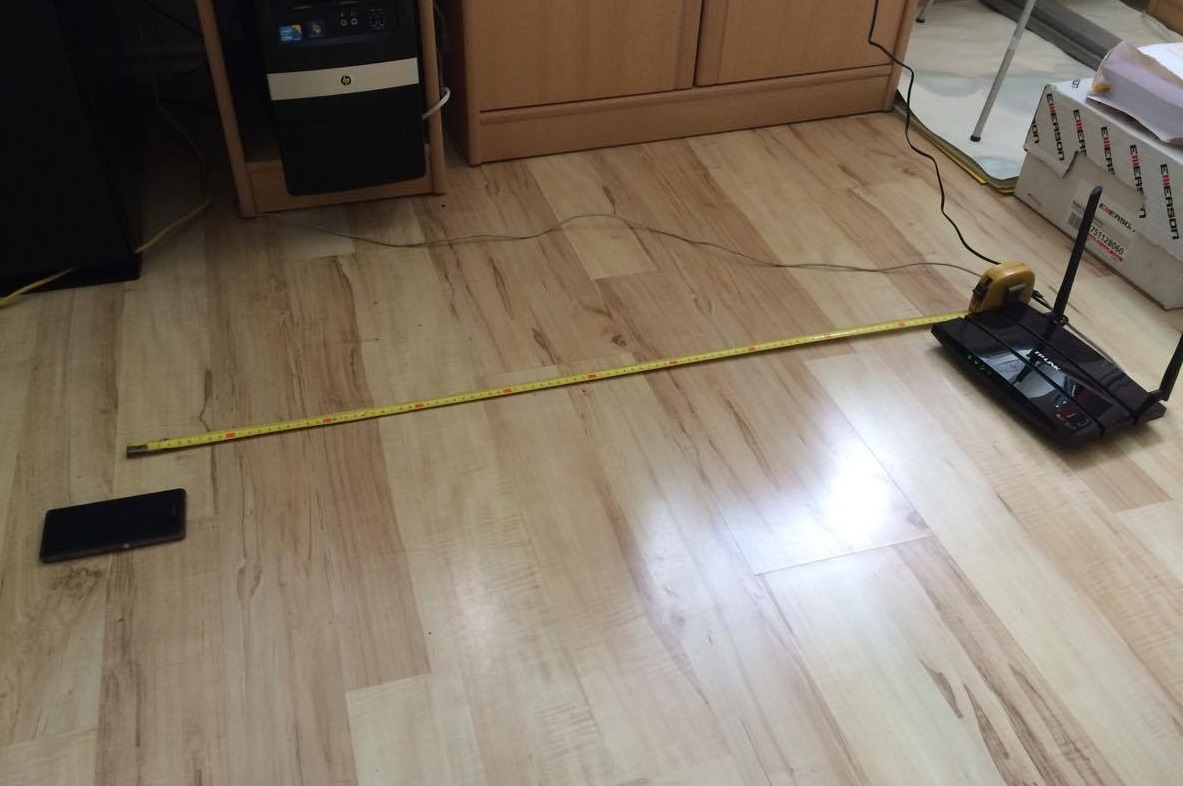
\includegraphics[width=0.75\textwidth]{srodowisko_pomiarowe}
\end{figure}
\section{Pobranie danych i analiza wyników}
Dla każdego eksperymentu została wykonana odpowiednio duża ilość powtórzeń (od 70 do 120), aby wynik był dokładniejszy. W tym celu, została stworzona lekka aplikacja, która pobierała zgłoszenia telefonu i zapisywała je do pliku tekstowego. Następnie, po skończonych testach, parsowała dane i wyliczała średnią dla sił sygnałów pochodzących z interesującego nas źródła (sygnały pochodzące z innych źródeł były odrzucane). Tak obliczone dane zostały zawarte w tabelach w dalszej części rozdziału (pełny wykaz danych uzyskanych podczas wykonywania eksperymentu znajduje się w dodatku "Appendix 1").
\section{Wyznaczenie wartości strat}
Eksperyment polegał na ustawieniu transmitera w odległości 1 metra od odbiornika, na jednym poziomie, antenami do siebie. Na podstawie siły sygnałów obliczana została wartość strat, jakie musiałyby być uwzględnione, aby odległość obliczona równała się odległości fizycznej.\\			
\begin{figure}[H]
	\centering			
	\caption{Szkic eksperymentu nr 1}
	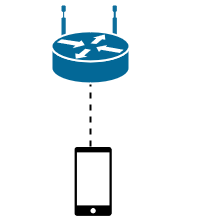
\includegraphics{exper1}
\end{figure}
\subsection{Pomiary}
	Wartości obliczone dla eksperymentu nr 1, w którym Router TP-Link TD-W8970 jest transmiterem sygnału Wifi, a Samsung Grand 2 transmiterem Bluetooth:
	\begin{center}
		\begin{minipage}{\linewidth}
			\begin{tabular}{|c|c|c|c|}
				\hline 
				Sygnał & Ilość prób & Średnia siła sygnału (w dBm) & Obliczona średnia wartość strat (dB) \\ 
				\hline 
				Wi-Fi & 163 & -38.88 & 21.18 \\ 
				\hline 
				Bluetooth & 113 & -57.5 & 23.3 \\ 
				\hline 
			\end{tabular} 
		\end{minipage} 
	\end{center}
\subsection{Wnioski}
Z danych uzyskanych podczas eksperymentu wynika, że straty spowodowane zakłóceniami sygnału Bluetooth są wyższe niż spowodowane zakłóceniami sygnału WiFi. Może się to wiązać z tym, że transmiter Wifi ma większą moc, zaś kierunkowe anteny zmniejszają ilość zakłóceń wynikających z odbicia się sygnału. Wartości strat obliczone dla obu sposobów komunikacji zostaną wykorzystane podczas eksperymentu nr 2 oraz będą miały wpływ na wybór wagi dla siły sygnałów podczas określania lokalizacji użytkowników.
\section{Przeszkody na drodze sygnału}
Drugi eksperyment ma na celu zbadanie odporności każdego z rodzajów sygnałów na zakłócenia związane ze stojącą na drodze przeszkodą. Wnioski z tego eksperymentu będą miały duży wpływ na działanie systemu, ponieważ w rzeczywistym środowisku, w którym ma działać tworzony system, transmiter od użytkownika będzie dzielić czasami nawet kilka ścian i ważne jest, aby odpowiednio dobrać wagi dla sygnałów.\\
W pierwszej części eksperymentu, transmiter został oddalony od odbiornika o 1 metr. Na drodze sygnału została postawiona gruba książka w formacie A4. W drugiej części eksperymentu, transmiter od odbiornika oddalony został o 2 metry, w taki sposób, aby na drodze sygnału znalazły się najpierw drewniane drzwi, a w kolejnej części eksperymentu ściana.\\
Do dokonania pomiarów zostały wykorzystane te same urządzenia jak w przypadku eksperymentu nr 1.\\
Wartość błędu bezwzględnego obliczana była na podstawie wzoru:
\begin{equation}
\delta = |D_r - D_o|
\end{equation}
gdzie $D_r$ to rzeczywista odległość między transmiterem, a odbiornikiem, zaś $D_o$ to odległość obliczona na podstawie siły sygnału.
\begin{figure}[H]
	\centering			
	\caption{Szkic eksperymentu nr 2}
	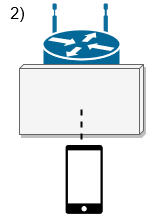
\includegraphics{exper2}
\end{figure}
\subsection{Pomiary}
Wartość siły sygnałów, obliczony dystans oraz wielkość błędu dla pomiaru sygnału Wifi i Bluetooth, dla którego przeszkodą była książka przy dystansie 1 metra:
\begin{center}
	\begin{minipage}{\linewidth}
		\begin{tabular}{|c|>{\centering\arraybackslash} p{2cm}|>{\centering\arraybackslash} p{3cm}|>{\centering\arraybackslash} p{3cm}|>{\centering\arraybackslash} p{2cm}|>{\centering\arraybackslash}p {2cm}|}
			\hline 
			Sygnał & Ilość pomiarów & Średnia siła sygnału (w dBm) & Średnia obliczona odległość (m) & Błąd bezwzględny (m) & Błąd względny (\%)\\
			\hline 
			Wifi & 182 & -40,81 & 1,24 & 0,24 & 24 \\ 
			\hline 
			Bluetooth & 70 & -61.46 & 1,57 & 0,57 & 57 \\ 
			\hline 			
		\end{tabular} 
	\end{minipage} 
\end{center}
Wartość siły sygnałów, obliczony dystans oraz wielkość błędu dla pomiaru sygnału Wifi i Bluetooth, dla którego przeszkodą były drzwi przy dystansie 2 metrów:
\begin{center}
	\begin{minipage}{\linewidth}
		\begin{tabular}{|c|>{\centering\arraybackslash} p{2cm}|>{\centering\arraybackslash} p{3cm}|>{\centering\arraybackslash} p{3cm}|>{\centering\arraybackslash} p{2cm}|>{\centering\arraybackslash}p {2cm}|}
			\hline 
			Sygnał & Ilość pomiarów & Średnia siła sygnału (w dBm) & Średnia obliczona odległość (m) & Błąd bezwzględny (m) & Błąd względny (\%)\\ 
			\hline 
			Wifi & 112 & -48,1 & 2,89 & 0,89 & 44,5\\ 
			\hline 
			Bluetooth & 107 & -67,05 & 3,01 & 1,01 & 50,5\\ 
			\hline 			
		\end{tabular} 
	\end{minipage} 
\end{center}
Wartość siły sygnałów, obliczony dystans oraz wielkość błędu dla pomiaru sygnału Wifi i Bluetooth, dla którego przeszkodą była ściana przy dystansie 2 metrów:
\begin{center}
	\begin{minipage}{\linewidth}
		\begin{tabular}{|c|>{\centering\arraybackslash} p{2cm}|>{\centering\arraybackslash} p{3cm}|>{\centering\arraybackslash} p{3cm}|>{\centering\arraybackslash} p{2cm}|>{\centering\arraybackslash}p {2cm}|}
			\hline 
			Sygnał & Ilość pomiarów & Średnia siła sygnału (w~dBm) & Średnia obliczona odległość (m) & Błąd bezwzględny (m) & Błąd względny (\%)\\ 
			\hline 
			Wifi & 103 & -48,3 & 2,96 & 0,96 & 48,0 \\ 
			\hline 
			Bluetooth & 110 & -66,95 & 2,97 & 0,97 & 48,5 \\ 
			\hline 			
		\end{tabular} 
	\end{minipage} 
\end{center}
\subsection{Wnioski}
Wyniki eksperymentu nr 2 jasno wskazują, że sygnał Wifi jest bardziej odporny na zmiany spowodowane pojawiającą się na drodze przeszkodą. Ma to duży wpływ na obliczanie lokalizacji użytkownika na podstawie sygnału i dlatego technologia Wifi będzie miała wyższą wagę w tworzonym systemie.\\
Dodatkowo, warto zwrócić uwagę, że błędy wynikające z obecności na drodze sygnału drzwi oraz ściany są mniejsze, niż można się było spodziewać. Może to wynikać z faktu, że sygnał nie rozchodzi się tylko w jednym kierunku i dzięki temu, podczas przechodzenia przez drzwi, część sygnału napotykała również na ścianę, co spowodowało większe zakłócenia.